\lecture{7}{}
\subsubsection*{两个随机变量的独立性}%
\label{subsub:两个随机变量的独立性}
\begin{proof}
    当$A,B$ 独立时:$P\left( AB \right) =P\left( A \right) P\left( B \right) $ 
    \[
        \forall i,j: P\left\{ X=x_{i},Y=y_{j} \right\} =P\left\{ X=x_{i} \right\} P\left( Y=y_{j} \right) 
    .\] 
\end{proof}
\begin{notation}
    离散随机变量独立的情况下:
    $P_{ij}=P_{i\cdot }\cdot P_{\cdot j}$ 

    如何证明$X,Y$ 独立:\[
        F\left( x,y \right) =P\left\{ X\le x,Y\le y \right\} =P\left\{ X\le x \right\} P\left\{ Y\le y \right\} =F_{X}\left( X \right) \cdot F_{Y}\left( y \right) 
    .\] 
\end{notation}
由联合分布律得边缘分布律:\[
    F_{X}\left( x \right) =\lim_{y \to +\infty} F\left( x,y \right) =\lim_{y_0 \to +\infty} P\left\{ X\le x,Y\le y_0 \right\} 
.\] 
\begin{notation}
    连续性随机变量的区间$D$概率:\[
        F\left( x,y \right) =P\left\{ X\le x,Y\le y \right\} =\iint_{u=x,v=y} f\left( u,v \right)  \mathrm{d}x\mathrm{d}y
    .\] 
\end{notation}

\subsubsection*{概率函数}%
\label{subsub:概率函数}
\begin{notation}
    二维均匀分布:
    \begin{align*}
        f\left( x,y \right) =\begin{cases}
            {\frac{1}{S\left( D \right) }},&\left( x,y \right) \in D\\
            0 ,& \left( x,y \right) \not\in D
        \end{cases}
    .\end{align*}
\end{notation}
\begin{eg}
    \begin{align*}
        f\left( x,y \right) =\begin{cases}
            Axy,&x\in \left( 0,1 \right) ,y\in \left( 0,1 \right) \\
            0,&\text{Others}
        \end{cases}
    .\end{align*}

    1. 求A
    \[
        \iint_{x\in [0,y] ,y\in [0,1] } Axy \mathrm{d}x\mathrm{d}y=1
    .\] 
    \begin{figure}[htpb]
        \centering
        \caption{$f\left( x,y \right) $}%
        \label{f( x,y )}
        \begin{tikzpicture}[yscale=1]
            % Axis
            \draw [->] (0,0)--(2,0) node [right] {$x$};
            \draw [->] (0,0)--(0,2) node [above] {$y$};
            \node [anchor=north east] at(0,0) {$O$};
    
            \draw [color=blue,semithick,domain=0:1] plot (\x, {\x});
            \draw [color=blue,semithick,domain=0:1] plot (\x,{1});
        \end{tikzpicture}
    \end{figure}

    $A=8$

    2. $P\left\{ X+Y\ge 1 \right\} $ 
    \begin{align*}
        P\left\{ X+Y\ge 1 \right\} &=\iint_{x+y\ge 1} f\left( x,y \right)  \mathrm{d}x\mathrm{d}y \\
        &= \iint_{x+y\ge 1} 8xy \mathrm{d}x\mathrm{d}y \\
        &= \int_{0.5}^{1} \mathrm{d}y \int_{1-y}^{y} 8xy \mathrm{d}x \\
        &= \frac{5}{6}
    .\end{align*}

    \begin{figure}[htbp]
        \centering
        \caption{$P(x+y\ge 1)$}
        \label{P(x+y>= 1)}
        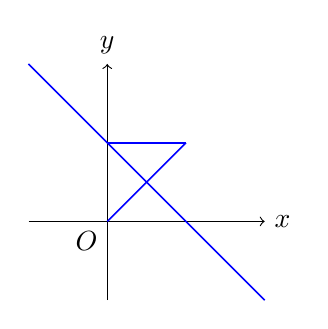
\begin{tikzpicture}[yscale=1]
            % Axis
            \draw [->] (-1,0)--(2,0) node [right] {$x$};
            \draw [->] (0,-1)--(0,2) node [above] {$y$};
            \node [anchor=north east] at(0,0) {$O$};
    
            \draw [color=blue,semithick,domain=0:1] plot (\x, {\x});
            \draw [color=blue,semithick,domain=0:1] plot (\x,{1});
            \draw [color=blue,semithick,domain=-1:2] plot (\x,{1-\x});
        \end{tikzpicture}
    \end{figure}

    3. $X,Y$ 的分布函数

    3.1 $x\in (-\infty,0), y\in (-\infty,0)$

    3.2 $x\in [0,1), y\in [0,x)$ 

    3.3 $x\in [0,1), y\in [x,1)$ 

    3.4 $x\in [0,1), y\in [1,+\infty)$ 

    3.5 $x\in [1,+\infty), y\in [0,1)$ 

    3.6 $x\in [1,+\infty), y\in [1,+\infty)$ 

    \begin{center}
        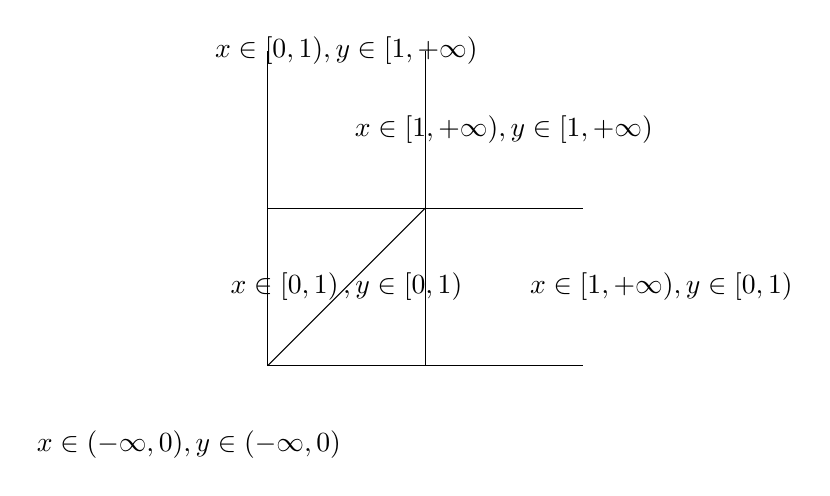
\begin{tikzpicture}
            \draw [] (-1,1) rectangle (1,-1) node at(0,0) {$x\in \left[ 0,1 \right) ,y\in \left[ 0,1 \right) $};
            \draw [] (1,1)--(3,1);
            \draw [] (1,1)--(1,3);
            \draw [] (-1,1)--(-1,3);
            \draw [] (1,-1)--(3,-1);
            \draw [] (-1,-1)--(1,1);
            \node [] at(2,2) {$x\in [1,+\infty),y\in [1,+\infty)$};
            \node [] at(-2,-2) {$x\in (-\infty,0),y\in (-\infty,0)$};
            \node [] at(4,0) {$x\in [1,+\infty),y\in [0,1)$};
            \node [] at(0,3) {$x\in [0,1),y\in [1,+\infty)$};
        \end{tikzpicture}
    \end{center}
    分段对$Axy$ 积分:
    \begin{align*}
        F\left( x,y \right) =\iint_{x\le u,y\le v} f\left( u,v \right)  \mathrm{d}x\mathrm{d}y
    \end{align*}
\end{eg}
\subsection{多维随机变量及分布}%
\label{sub:多维随机变量及分布}
\begin{defi}
    二维推广至多维:
    \[
        F\left( x_1,x_2,\cdots,x_n \right) =P\left\{ X_1\le x_1,X_2\le x_2,\cdots,X_n\le x_n \right\} 
    .\] 

    称$F$ 为$n$ 维随机变量的联合分布函数
\end{defi}
\begin{defi}
    多维联合分布律:
    \[
        P\left\{ X_1=a_{1k_1},X_2=a_{2k_2},\cdots,X_n=a_{nk_n} \right\} 
    .\] 
\end{defi}
联合分布函数和联合分布律的关系:\[
    F\left( x_1,x_2,\cdots,x_n \right) 
.\]
\[
    =\sum_{a_{1k_1}\le x_1}\sum_{a_{2k_2}\le x_2}\cdots \sum_{a_{nk_n}\le x_{n}} P\left\{ X_1=a_{1k_1},X_2=a_{2k_2},\cdots,X_n=a_{nk_n} \right\} 
.\] 
\begin{notation}
    二项分布推广多项分布:

    $A_1,A_2,\cdots,A_r$是$E$ 的完备事件组,$P\left( A_i \right) =p_i,i=1,2,\cdots,r$,对$E$ 进行$n$ 次独立重复试验,$X_{i}$ 表示$A_{i}$ 发生的次数,则:\[
        P\left\{ X_1=k_1,X_2=k_2,\cdots,X_r=k_r \right\} =\frac{n!}{k_1!k_2!\cdots k_r!}\prod_{i=1}^{r} p_{i}^{k_i} 
    .\] 

    其中$k_i\ge 0,{\sum_{i=1}^{r} k_i=n}$,当$n=2$ 时为二项分布
\end{notation}

\subsubsection{多维随机变量的独立性}%
\label{subsub:多维随机变量的独立性}
\begin{defi}
    \[
        F\left( x_1,x_2,\cdots,x_n \right) =\prod_{i=1}^{n} F_{X_i}\left( x_i \right) 
    .\] 

    称随机变量相互独立

    等价于:\[
        f\left( x_1,x_2,\cdots,x_n \right) =\prod_{i=1}^{n} f_{X_i}\left( x_i \right)  
    .\] 
\end{defi}

